% Presentation slides for the IT4130E group project.
% Compile:  latexmk -pdf slides.tex   or   tectonic slides.tex
\documentclass[aspectratio=169]{beamer}
\usetheme{Madrid}
\usecolortheme{seahorse}
\setbeamertemplate{navigation symbols}{}

\usepackage{booktabs}
\usepackage{amsmath}
\usepackage{graphicx}
\usepackage{algorithm}
\usepackage{algpseudocode}
\usepackage{tikz}

\graphicspath{{figures/}}

\title[Parallel Barnes--Hut $N$-body]{Distributed-Memory Parallelisation of a
Barnes--Hut $N$-Body Simulation}
\subtitle{IT4130E Parallel and Distributed Programming}
\author[Group]{\textit{[member 1] \and [member 2] \and [member 3] \and [member 4]}}
\institute{\textit{[instructor name]}}
\date{\today}

\begin{document}

\begin{frame}\titlepage\end{frame}

\begin{frame}{Outline}\tableofcontents\end{frame}

% ------------------------------------------------------------------
\section{Problem}
\begin{frame}{The $N$-body problem}
\begin{columns}
\begin{column}{0.58\textwidth}
\begin{itemize}
  \item $N$ masses attract each other by Newtonian gravity; advance their
        motion through time.
  \item Force on a body sums contributions of all others:
        \[ \vec a_i = G\sum_{j\neq i} m_j\,
           \frac{\vec r_j-\vec r_i}{(\lVert\vec r_j-\vec r_i\rVert^2+\varepsilon^2)^{3/2}} \]
  \item Direct evaluation costs $\mathcal{O}(N^2)$ per step --- too slow.
  \item \textbf{Goal:} a correct sequential method, a distributed-memory (MPI)
        parallel version, and a hybrid MPI\,+\,OpenMP version, with a measured
        performance study.
\end{itemize}
\end{column}
\begin{column}{0.42\textwidth}
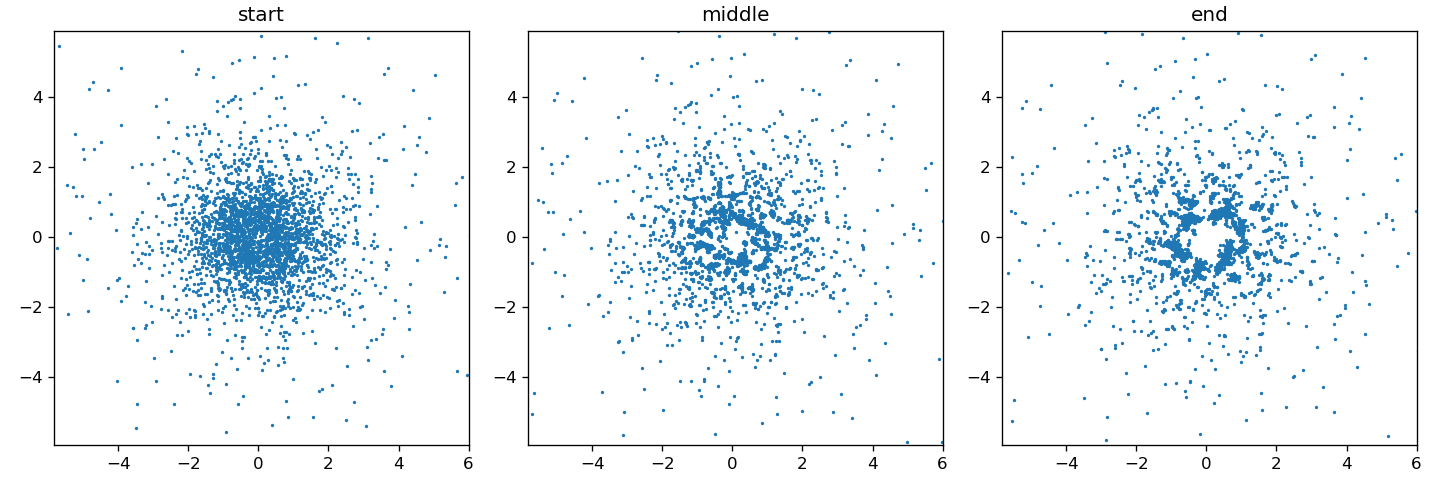
\includegraphics[width=\linewidth]{sim.png}
\end{column}
\end{columns}
\end{frame}

\begin{frame}{Barnes--Hut: $\mathcal{O}(N\log N)$}
\begin{columns}
\begin{column}{0.6\textwidth}
\begin{itemize}
  \item Recursively divide the plane into a \textbf{quadtree}; each leaf holds
        $\le 1$ body.
  \item Each node stores the total mass and centre of mass below it.
  \item Force on a body: traverse from the root. If a node is far enough
        ($s/d<\theta$), treat the whole subtree as one mass; else descend.
  \item $\theta=0.5$: about $1\%$ force error, $\mathcal{O}(N\log N)$ work.
  \item The tree makes the work \textbf{irregular} --- the key parallel
        challenge.
\end{itemize}
\end{column}
\begin{column}{0.4\textwidth}
\centering
\footnotesize
$s/d < \theta \Rightarrow$ approximate\\[4pt]
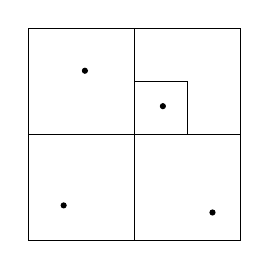
\begin{tikzpicture}[scale=0.9]
  \draw (0,0) rectangle (3,3);
  \draw (1.5,0)--(1.5,3); \draw (0,1.5)--(3,1.5);
  \draw (1.5,1.5) rectangle (2.25,2.25);
  \filldraw (1.9,1.9) circle (1pt);
  \filldraw (0.5,0.5) circle (1pt); \filldraw (0.8,2.4) circle (1pt);
  \filldraw (2.6,0.4) circle (1pt);
\end{tikzpicture}
\end{column}
\end{columns}
\end{frame}

% ------------------------------------------------------------------
\section{Parallelisation}
\begin{frame}{Design choices (the rubric questions)}
\begin{itemize}
  \item \textbf{Level of parallelism:} \emph{data} --- same operation, different
        bodies.
  \item \textbf{Decomposition:} \emph{data decomposition} (owner-computes per
        body) over a \emph{recursive} (replicated) tree build $\Rightarrow$
        hybrid, data-dominated.
  \item \textbf{Mapping:} \emph{1-D block} --- process $r$ owns a contiguous block
        of $\approx N/P$ bodies (not 2-D $\sqrt{P}\times\sqrt{P}$: the domain is a
        1-D list, not a grid).
  \item \textbf{Communication:} \emph{blocking, collective}; broadcast once at
        start, then one \emph{all-gather} of positions per step. Symmetric
        single-program multiple-data (SPMD),
        \emph{no} master--slave; no explicit ring/hypercube topology.
  \item \textbf{Load balance:} equal block \emph{size}; work per body is uneven
        (dense regions cost more).
\end{itemize}
\end{frame}

\begin{frame}{Parallel algorithm (process $r$ of $P$)}
\begin{algorithmic}[1]
\State \textbf{(once)} broadcast initial positions, velocities, masses
\State $lo,hi \gets$ block owned by process $r$ \Comment{1-D block}
\For{each time step}
  \State build the full quadtree locally \Comment{replicated}
  \State accumulate mass / centre of mass at each node
  \For{$i = lo \dots hi-1$} \Comment{OpenMP parallel-for in hybrid}
     \State $\vec a_i \gets$ traverse tree with $\theta$
  \EndFor
  \State $\vec v_i \mathrel{+}= \vec a_i\Delta t$; \; $\vec r_i \mathrel{+}= \vec v_i\Delta t$
  \State \textbf{all-gather} updated positions
\EndFor
\end{algorithmic}
\vspace{4pt}
\footnotesize Force traversal communicates nothing (tree is complete on every
process). Cost: build $\mathcal{O}(N)$ replicated $+$ force
$\mathcal{O}((N/P)\log N)$ $+$ comm $\mathcal{O}(N)$.
\end{frame}

% ------------------------------------------------------------------
\section{Results}
\begin{frame}{Correctness}
\begin{itemize}
  \item Parallel and hybrid outputs match the sequential reference \textbf{bit for
        bit}, for every process and thread count tested.
  \begin{itemize}\footnotesize
    \item Each body is integrated by identical arithmetic; the all-gather moves
          data without changing it.
  \end{itemize}
  \item Total energy conserved to within a fraction of a percent over the run
        $\Rightarrow$ the model is physically stable.
  \item The cluster stays bound and near equilibrium (title figure).
\end{itemize}
\end{frame}

\begin{frame}{Running time vs problem size (choosing $N$)}
\begin{columns}
\begin{column}{0.55\textwidth}
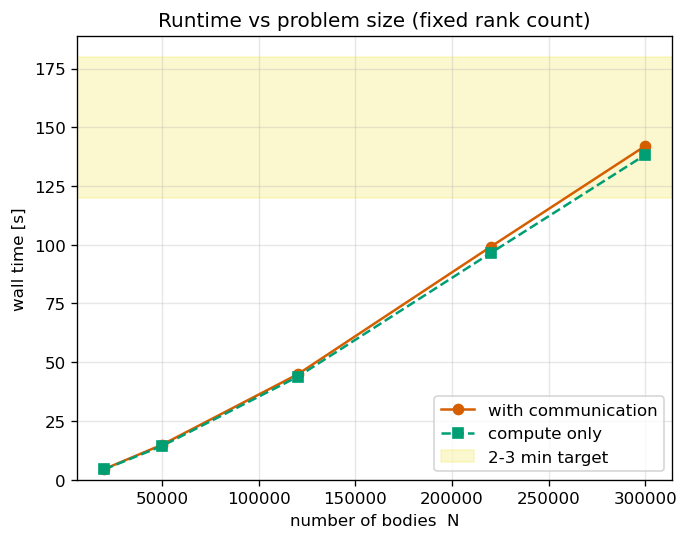
\includegraphics[width=\linewidth]{scaling_n.png}
\end{column}
\begin{column}{0.45\textwidth}
\begin{itemize}
  \item Twelve processes (= cores), vary $N$.
  \item Time grows $\sim N\log N$; communication is a small fraction.
  \item Pick the $N$ landing in the 2--3 minute band as the operating point for
        the load-balance study.
\end{itemize}
\end{column}
\end{columns}
\end{frame}

\begin{frame}{Granularity \& load balance (25\% idle rule)}
\begin{columns}
\begin{column}{0.5\textwidth}
\centering Balanced (generated order)\\
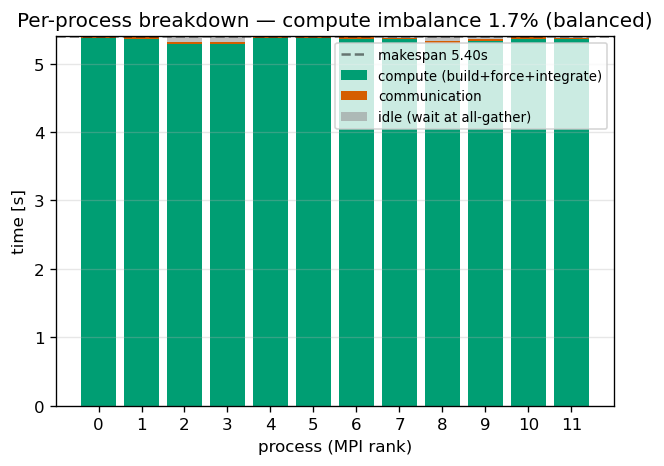
\includegraphics[width=\linewidth]{granularity_balanced.png}
\end{column}
\begin{column}{0.5\textwidth}
\centering Imbalanced (sorted by position)\\
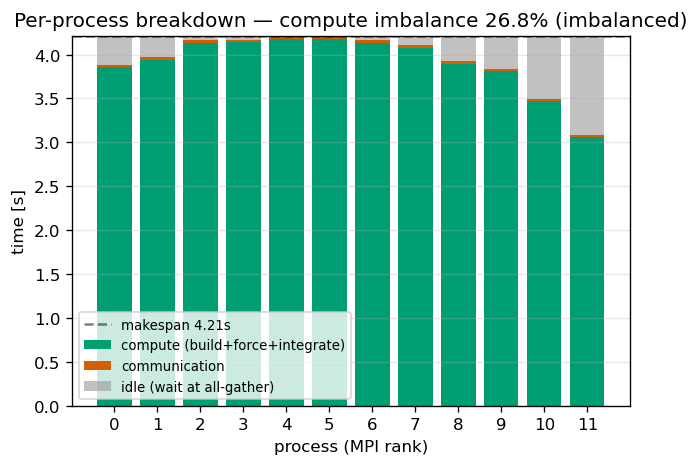
\includegraphics[width=\linewidth]{granularity_imbalanced.png}
\end{column}
\end{columns}
\vspace{2pt}
\footnotesize Equal block \emph{size} $=$ equal \emph{work} only when ordering is
unrelated to position. Fix: cyclic distribution / dynamic thread schedule.
\end{frame}

\begin{frame}{Speed-up}
\begin{columns}
\begin{column}{0.5\textwidth}
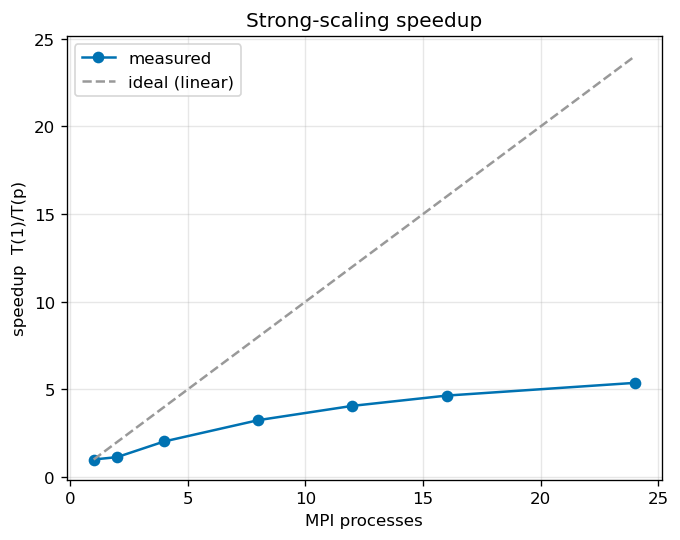
\includegraphics[width=\linewidth]{speedup.png}
\end{column}
\begin{column}{0.5\textwidth}
\begin{itemize}
  \item Fixed size, double the processes $1,2,4,\dots,2X$.
  \item Speed-up saturates: the \textbf{replicated tree build} is not divided
        $\Rightarrow$ Amdahl ceiling.
  \item Communication is the second, smaller cost (gap between runtime curves).
\end{itemize}
\end{column}
\end{columns}
\end{frame}

% ------------------------------------------------------------------
\section{Conclusion}
\begin{frame}{Conclusion}
\begin{itemize}
  \item Data-parallel Barnes--Hut: force work divides cleanly and communicates
        nothing; result is identical to sequential.
  \item Clear speed-up, with an efficiency ceiling \emph{explained} by the
        replicated build (Amdahl) and the per-step all-gather.
  \item Load balance follows directly from the mapping and the input ordering.
  \item \textbf{Future work:} distribute the tree (remove the sequential build),
        cyclic / cost-aware mapping, extend to 3-D (octree).
\end{itemize}
\vspace{6pt}
\centering\large Thank you --- questions?
\end{frame}

\end{document}
